\documentclass[tikz]{standalone}

\usepackage[latin1]{inputenc}
\usepackage{tikz}

\begin{document}
\pagestyle{empty}

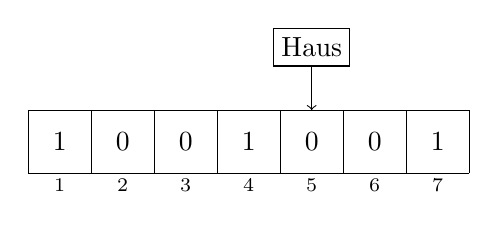
\begin{tikzpicture}[scale=0.8]
    \draw (0.9,-0.3) rectangle (2.1,0.3);
    \node at (1.5,0) {Haus};
    \draw (-3,-2) grid (4,-1);
    \draw[->] (1.5,-0.3) -- (1.5,-1);

    \node at (-2.5,-1.5) {$1$};
    \node at (-1.5,-1.5) {$0$};
    \node at (-0.5,-1.5) {$0$};
    \node at (0.5,-1.5) {$1$};
    \node at (1.5,-1.5) {$0$};
    \node at (2.5,-1.5) {$0$};
    \node at (3.5,-1.5) {$1$};

    \node at (-2.5,-2.2) {\scriptsize $1$};
    \node at (-1.5,-2.2) {\scriptsize $2$};
    \node at (-0.5,-2.2) {\scriptsize $3$};
    \node at (0.5,-2.2) {\scriptsize $4$};
    \node at (1.5,-2.2) {\scriptsize $5$};
    \node at (2.5,-2.2) {\scriptsize $6$};
    \node at (3.5,-2.2) {\scriptsize $7$};

    % \def\size {5}
    % \def\cellscale {1.5}
    % \foreach \x in {0,...,\size}
    %     \foreach \y in {\size,...,0}
    %     {
    %         \draw (\cellscale*\x,\cellscale*\y) rectangle +(\cellscale, \cellscale);
    %         \draw (\cellscale*\x + \cellscale/2,\cellscale*\y + \cellscale/2) node{$(\y,\x)$};
    %     }
\end{tikzpicture}
\end{document}
